\subsection{Singleton}
Viene utilizzato quando si vuole assicurare l'esistenza di un'unica istanza di una determinata classe e si vuole fornire un unico punto d'accesso globale a questa istanza.
\begin{figure}[ht]
    \centering
    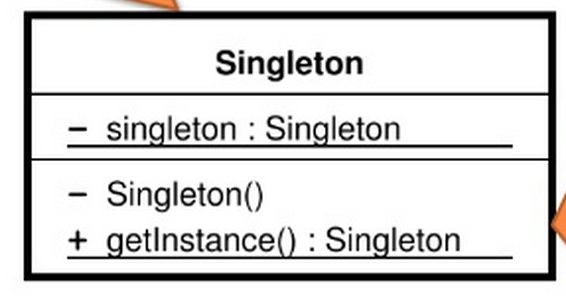
\includegraphics[width=0.8\textwidth]{immagini/singleton.png}
    \caption{Singleton}
\end{figure}
\FloatBarrier
La classe viene quindi definita con un costruttore privato e l'unico modo per crearla è tramite un metodo pubblico, che, controlla se esiste già un'istanza e nel caso esista, ritorna un riferimeto a quell'istanza anziché creare un nuovo oggetto.
Utilizzando questo pattern si riesce ad avere un controllo completo sul numero di istanze presenti e sul come i vari client possono accedervi, evitando l'utilizzo di variabili globali e rendendo possibile applicare anche il polimorfismo.